\section{Experimental validation}
\label{sec:expe}

\subsection{Methodology}
\label{sec:exp-methodo}

This section briefly discusses our experimental setup for the evaluation of
\Moca.

All our experiment were run on  machines from Grid5000 \emph{Edel} cluster
\footnote{A full hardware description is available here
    \url{https://www.grid5000.fr/mediawiki/index.php/Grenoble:Hardware\#Edel}}.
    These machines are composed of $2$ quad core \texttt{Intel Xeon E5520}
    cadenced a $2.27GHz$ with
    $24 GB$ of RAM. Hyper threading was disabled during the experiment.

We deployed a \emph{Debian} \emph{Wheezy} environment running a Linux $3.X$
\DB{Linux version}.
\DB{Environment online ?}.
\DB{Results online ?}

We evaluate our tool on all the NAS Parallel Benchmarks~\cite{Jin1999} for
each benchmarks, we compare \Moca with the Pin~\cite{Luk05Pin} instrumentation
from Tabarnac~\cite{Beniamine15TABARNACRR}. This instrumentation traces every
memory accesses but record only the number of time each thread accesses to
each page, without any other information.

Each configuration of each plots was executed at least $32$ times. Each point
shows the arithmetic mean of all runs. The error bars represent
the standard error.

Except for the experiment on the influence of \Moca's parameters, on every
experiment, \Moca was run with it's default parameters. Which are a logging
process wakeup interval of $0.5s$ and a monitor thread wakeup interval
of $40ms$.


\subsection{Experiments}
\label{sec:expe-ovh}

\subsubsection{\Moca default parameters}

\begin{figure}[htb]
    \centering
    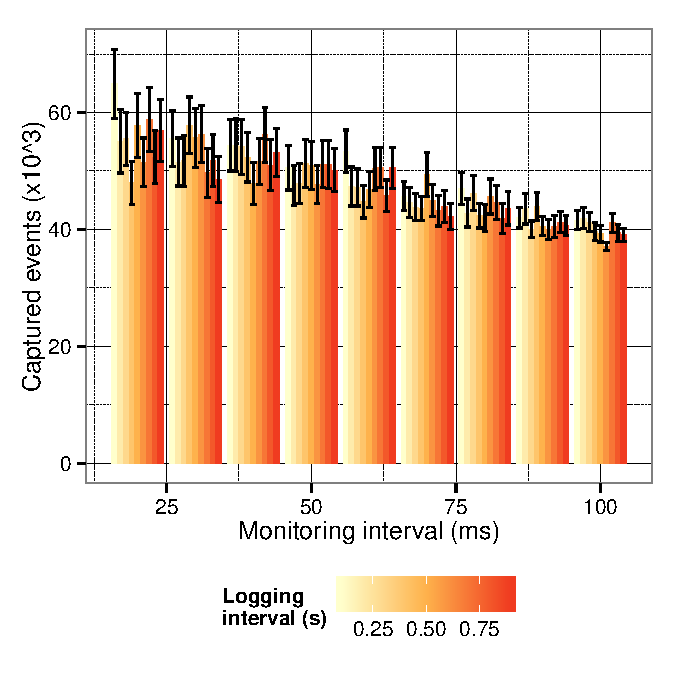
\includegraphics[width=\linewidth]{moca_param_events.pdf}
    \caption{Influence of the wakeup intervals on \Moca's the number of
    captured events on \FT, class A.}
    \label{fig:param_evts}
\end{figure}

Before comparing \Moca to existing tools, we need to evaluate the impact of
the wakeup intervals (logging daemon and monitor thread) on the trace
precision and on the overhead. To do so, we run the \FT under \Moca with
a wakeup interval from $0.1s$ to  $0.9s$ for the logging daemon and $20ms$ to
$100ms$. For each run, we measured \FT execution time and the number of
accesses captured.

\begin{figure}[htb]
    \centering
    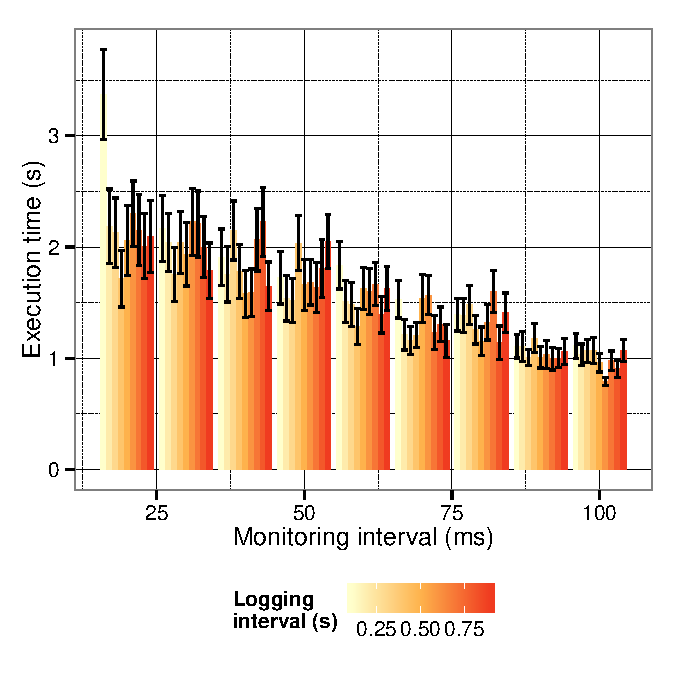
\includegraphics[width=\linewidth]{moca_param.pdf}
    \caption{Influence of the wakeup intervals on \Moca's overhead on
        \FT, class A.}
    \label{fig:param}
\end{figure}

We can see in Figure~\ref{fig:param_evts} that when the monitor thread wakes
up less often then every $40ms$ the number of captured event start to drops.
Moreover, Figure~\ref{fig:param} show that if the performance are decreasing
start with a monitor thread wakeup interval of $40ms$, there is a sweet spot
with a logging interval of $0.4ms$.
    \DB{Only 20 runs, here intervals should be smaller on definitive version}

Using this knowledge, we set the default wakeup intervals to $40ms$ for the
monitor thread, and $0.4s$ for the logging thread.

\subsubsection{Comparison with existing tools}

\begin{figure}[htb]
    \centering
    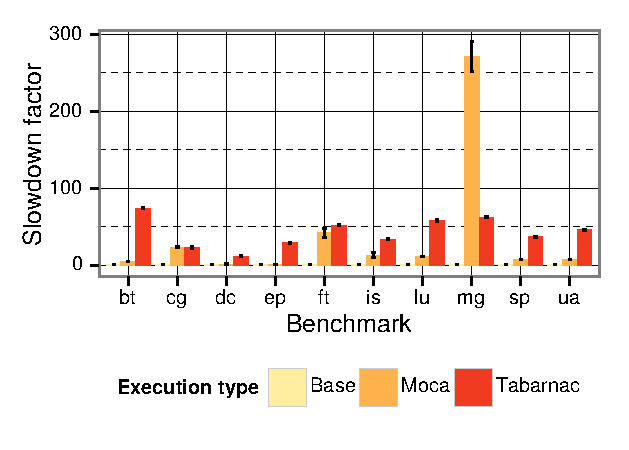
\includegraphics[width=\linewidth]{moca_overhead_nas.pdf}
    \caption{Slowdown of \Moca on the NAS parallel benchmarks compared to
    Tabarnac.}
    \label{fig:ovh}
\end{figure}

\begin{figure}[htb]
    \centering
    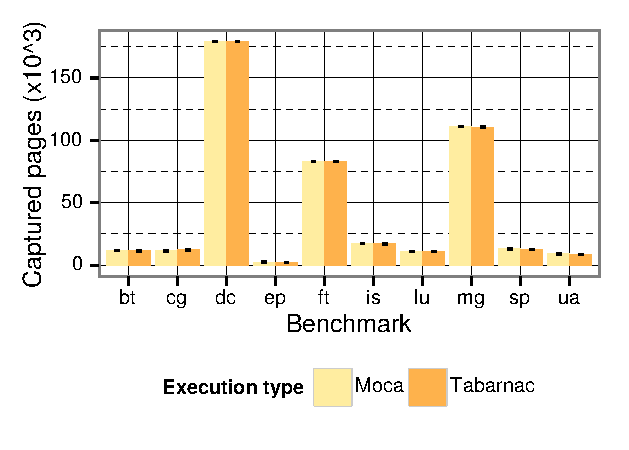
\includegraphics[width=\linewidth]{moca_pages_nas.pdf}
    \caption{Number of pages captured by \Moca and Tabarnac on the Nas
    Parrallel benchmarks.}
    \label{fig:pages}
\end{figure}

\begin{figure}[htb]
    \centering
    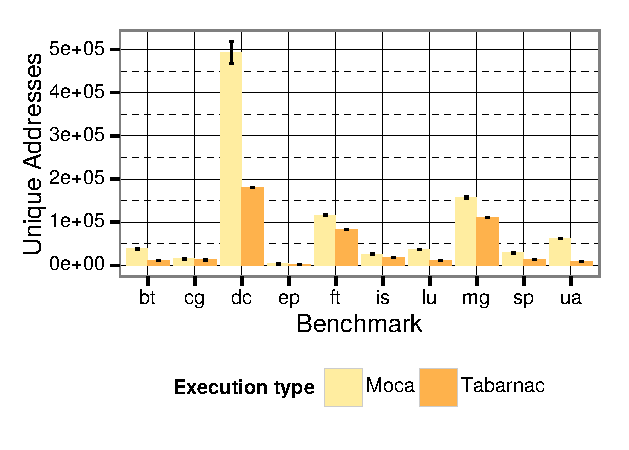
\includegraphics[width=\linewidth]{moca_addresses_nas.pdf}
    \caption{Number of unique addresses captured by \Moca and Tabarnac on the Nas
    Parrallel benchmarks.}
    \label{fig:addr}
\end{figure}

\begin{itemize}
    \item Wakeup and logging interval => define defaults Figure~\ref{fig:param}
    \item NAS + Tabarnac => not worst than other tools Figure~\ref{fig:ovh}
    \item Number of Pages => No loss Figure~\ref{fig:pages}
    \item Number of uniq address => More precise Figure~\ref{fig:addr}
    \item Trace details see Table~\ref{tab:tools-comp}
\end{itemize}

    \subsection{Conclusion}
    \label{sec:expe-cncl}

    \begin{itemize}
        \item ``fast''
        \item ``precise''
    \end{itemize}
